\typeout{NT FILE EVAL.tex}%
\chapter{Evaluation}
\label{cha:evaluation}

\section{Functional tests}
\label{sec:functional-tests}
Fig.~\ref{fig:uav-main-eval-kmod} shows an overview of the functional
tests. The basic idea is to assess the behavior of the system in case a
malicious actor gains access to the system and hijacks it. 
To emulate this scenario, we deployed a malicious software component -- running
on user space (\lstinline{crash_app}) or in kernel space (\lstinline{crash_mod.ko})
-- to the \gls{uavic} platform in both unsupervised and
supervised cases. In the \textbf{unsupervised}
test the malicious component is loaded on top of the Linux \gls{os} (1) causing
a system crash (2), which catastrophically terminates both non-critical (video
surveillance) and critical (PX4) software stacks and, consequently, leads to the
\gls{uav} failure. In the \textbf{supervised} test, the malicious component is deployed to the Companion \gls{vm} (1), triggering a
hypervisor fault (2), which causes the \gls{vm} crash. However, now, only the
non-critical software stack (video) is terminated, while the critical-one (PX4),
and consequently, the \gls{uav} remains on and operational.

\begin{figure}[!hbt]
  \centering
  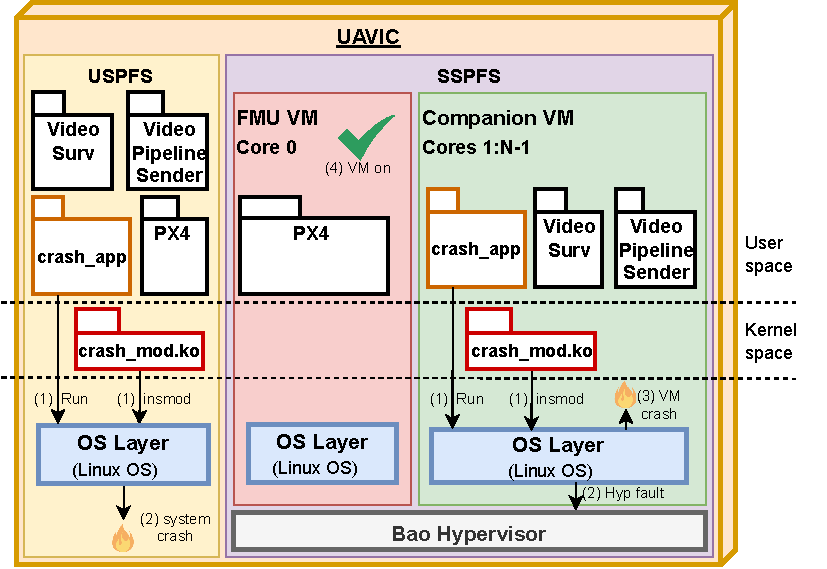
\includegraphics[width=0.8\textwidth]{./img/pdf/uav-main-eval-funcTest} 
%  \includesvg[width=1.0\textwidth]{./img/virtualization.svg} 
  %\caption[Virtualization mind map]{Virtualization mind map}%
  \caption{Functional tests' overview}%
  \label{fig:uav-main-eval-kmod}
\end{figure}

\subsection{Privileged mode}
\label{sec:privileged-mode}
The malicious actor may be able to gain access to the system and remotely
execute code in privileged mode, i.e., running as super user or directly in the
kernel space. In this section, we explore several approaches to crash the system
through the execution of a malicious kernel module.

\subsubsection{Panic}
\label{sec:panic}
One of the simplest methods to crash the system using a kernel module is to
explicitly invoke a \lstinline{panic}, signalling to the system an unrecoverable
state has been reached. Listing~\ref{lst:kmod-panic} depicts this approach, namely
line 5. When executing, the \lstinline{panic} function will~\cite{panicLinux}: (1) disable local
interrupts and preemption; (2) identify the ``panic master CPU`` and force all
other \glspl{cpu} to halt; (3) add the message 
\lstinline{Forced kernel panic!} to the kernel ring message, which can be inspected using a tool
such as \lstinline{dmesg}; (4) if a timeout is set, the system will reboot after
it expires; (5)
else, the system enters an infinite loop freezing the system.

\begin{longlisting}
\centering
\inputminted[]{c}{./listing/kmod_panic.c}
\caption{Functional tests: implementation of the Panic kernel module}
\label{lst:kmod-panic}
\end{longlisting}

Fig.~\ref{fig:kmod-panic-test} shows the panic kernel module testing for the
\gls{uspfs} system. In the top
left window is the \gls{uart} connection used to boot the system (1). Then, in
the top right window, we
connect remotely to \gls{uspfs} system using \gls{ssh} over Wi-Fi and we insert
the malicious kernel module (2). We can observe in the bottom window we cannot
\lstinline{ping} the system in the network (3), as it is not online
anymore. Hence, this would translate to a catastrophic failure of the \gls{uav}.

\begin{figure}[!hbt]
  \centering
  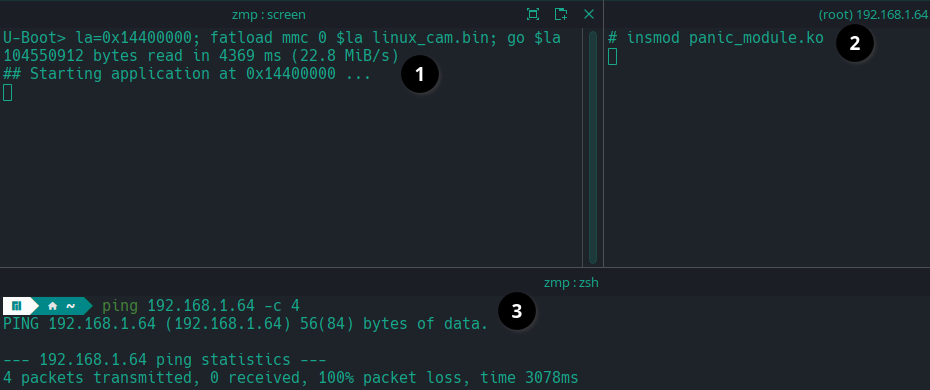
\includegraphics[width=1.0\textwidth]{./img/png/kmod-panic-test-annot} 
  \caption{Functional tests: Panic kernel module testing -- USPFS}%
  \label{fig:kmod-panic-test}
\end{figure}

Fig.~\ref{fig:kmod-panic-test-bao} shows the panic kernel module testing for the
\gls{sspfs} system. In the top
left window is the \gls{uart} connection used to boot the system (1), which is
shared also between Bao and the PX4 \gls{vm}. Then, in
the top right window, we connect remotely to Companion \gls{vm} using \gls{ssh} over Wi-Fi and we insert
the malicious kernel module (2). We can observe in the bottom window we cannot
\lstinline{ping} the Companion \gls{vm} in the network (3), as it is not online
anymore. However, we can still interact with the PX4 \gls{vm} (4), as the
Companion \gls{vm} crash does not propagate to the PX4 \gls{vm}, hence, the
\gls{uav} remains on and operational. Thus, it was
demonstrated that the Bao hypervisor allows for consolidation of the
mixed-criticality software stacks
into a single platform while providing isolation between these
domains.

\begin{figure}[!hbt]
  \centering
  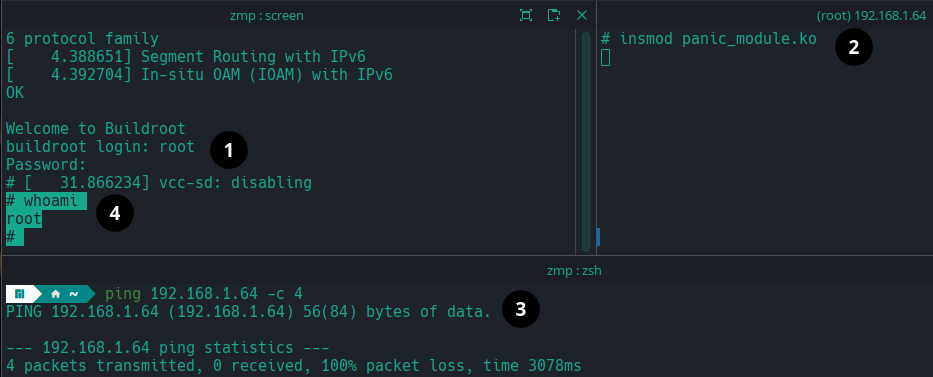
\includegraphics[width=1.0\textwidth]{./img/png/kmod-panic-test-bao-annot} 
  \caption{Functional tests: Panic kernel module testing -- SSPFS}%
  \label{fig:kmod-panic-test-bao}
\end{figure}


\subsubsection{Memory corruption}
\label{sec:mem-corrupt}
Another approach to crash the system is to write to unmapped/inexistent physical
memory addresses. Listing~\ref{lst:kmod-memcorrupt} depicts this approach, which was
made parameterizable for easier testing (lines 9 -- 10). We map a valid, but inexistent, physical
address to the kernel virtual address (line 27) and write data to it (line 36),
which triggers a crash, as the virtual address is not backed up by an existent
physical address~\cite{iomapLinux}.

\begin{longlisting}
\centering
\inputminted[]{c}{./listing/kmod_memcorrupt.c}
\caption{Functional tests: implementation of the Memory Corruption kernel module}
\label{lst:kmod-memcorrupt}
\end{longlisting}

Fig.~\ref{fig:kmod-memcorrupt-test} shows the testing of the memory corruption kernel
module for \gls{uspfs} system. In the top
left window is the \gls{uart} connection used to boot the system (1). Then, in
the top right window, we
connect remotely to \gls{uspfs} system using \gls{ssh} over Wi-Fi and we insert
the malicious kernel module (2), passing the inexistent address \lstinline{0x8_0000_0000}
as an argument. This address exceeds the physical address range for the
Raspberry Pi 4 (\lstinline{0x7_FFFF_FFFF}~\cite{rpi4-bcm2711}). We can observe in the bottom window we cannot
\lstinline{ping} the system in the network (3), as it is not online
anymore. Hence, this would translate to a catastrophic failure of the \gls{uav}.

\begin{figure}[!hbt]
  \centering
  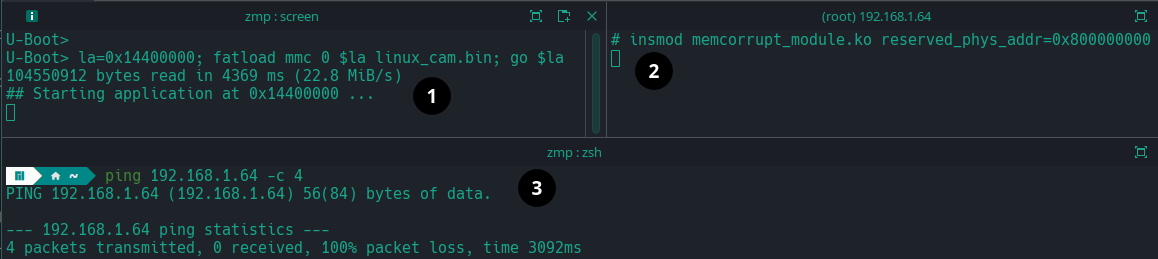
\includegraphics[width=1.0\textwidth]{./img/png/kmod-memcorrupt-test-annot} 
  \caption{Functional tests: testing of the memory corruption kernel module -- USPFS}%
  \label{fig:kmod-memcorrupt-test}
\end{figure}

Fig.~\ref{fig:kmod-memcorrupt-test} shows the testing of the memory corruption kernel
module for \gls{sspfs} system. In the top
left window is the \gls{uart} connection used to boot the system (1), which is
shared also between Bao and the PX4 \gls{vm}. Then, in
the top right window, we connect remotely to Companion \gls{vm} using \gls{ssh} over Wi-Fi and we insert
the malicious kernel module (2), passing the inexistent address \lstinline{0x8_0000_0000}
as an argument. This causes the Companion VM to crash, triggering a hypervisor
fault at the corresponding virtual address (3). We can observe in the bottom window we cannot
\lstinline{ping} the Companion \gls{vm} in the network (4), as it is not online
anymore. However, we can still interact with the PX4 \gls{vm} (5), as the
Companion \gls{vm} crash does not propagate to the PX4 \gls{vm}, hence, the
\gls{uav} remains on and operational. 

\begin{figure}[!hbt]
  \centering
  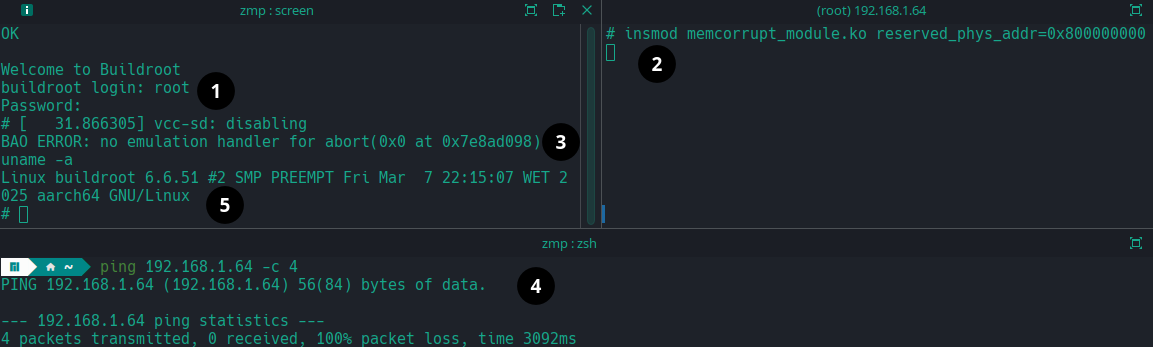
\includegraphics[width=1.0\textwidth]{./img/png/kmod-memcorrupt-test-bao-annot} 
  \caption{Functional tests: testing of the memory corruption kernel module -- SSPFS}%
  \label{fig:kmod-memcorrupt-test-bao}
\end{figure}

\subsubsection{Memory exhaustion}
\label{sec:mem-exhaustion}
Another viable method to crash the system is to exhaust all system's memory (see
Listing~\ref{lst:kmod-memhog}). Firstly, we adjust the \gls{oom} score of the
current process (i.e., the kernel thread running this module) to the minimum
value. By doing so, it makes this process less likely to be targeted by the
\gls{oom} killer when the system runs low on memory (line 9). The module then
enters an infinite loop (line 11), where it repeatedly allocates a single memory
page, which is locked (line 16) to prevent it from being freed. Thus, the memory
is ``hogged`` permanently by this module, ensuring it is not reclaimed even
under memory pressure.

\begin{longlisting}
\centering
\inputminted[]{c}{./listing/kmod_memhog.c}
\caption{Functional tests: implementation of the Memory Exhaustion kernel module}
\label{lst:kmod-memhog}
\end{longlisting}

Fig.~\ref{fig:kmod-memhog-test} and Fig.~\ref{fig:kmod-memhog-test-bao} show the
testing of the memory exhaustion kernel module for the \gls{uspfs} and
\gls{sspfs} system, respectively. Once again, it can be observed that the
system's crash is catastrophic for the \gls{uspfs} system, but not for the
\gls{sspfs} one.

\begin{figure}[!hbt]
  \centering
  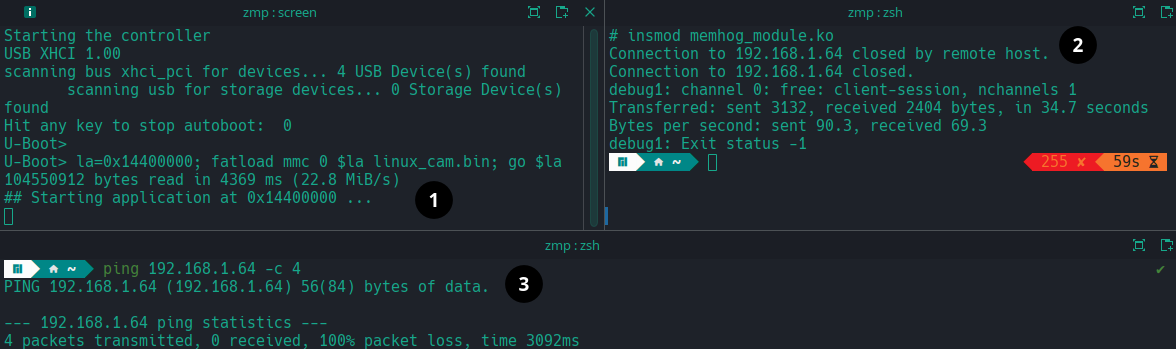
\includegraphics[width=1.0\textwidth]{./img/png/kmod-memhog-test-annot} 
  \caption{Functional tests: testing of the memory exhaustion kernel module -- USPFS}%
  \label{fig:kmod-memhog-test}
\end{figure}

\begin{figure}[!hbt]
  \centering
  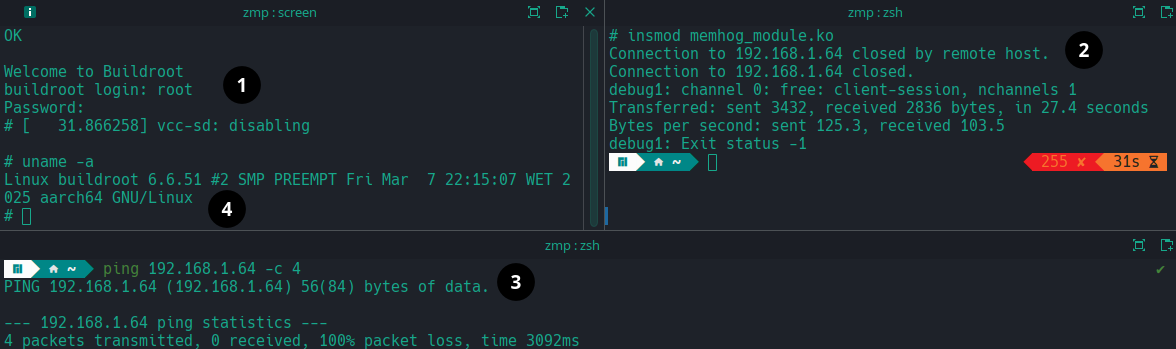
\includegraphics[width=1.0\textwidth]{./img/png/kmod-memhog-test-bao-annot} 
  \caption{Functional tests: testing of the memory exhaustion kernel module -- SSPFS}%
  \label{fig:kmod-memhog-test-bao}
\end{figure}


\subsubsection{Kill init process}
\label{sec:kill-init-process}
Lastly, we can crash the system by killing the \lstinline{init} process (see
Listing~\ref{lst:kmod-initkiller}). Firstly, we retrieve a reference to the
\lstinline{init} process (line 16) and its memory layout (line 19). We then
iterate over all \glspl{vma} (line 25) and, for each page (line 27) we pin it to
prevent it from being swapped (line 32), and we corrupt its data (line 38). By
doing so, we effectively corrupt all data associated to the \lstinline{init}
process, causing a system crash.

\begin{longlisting}
\centering
\inputminted[]{c}{./listing/kmod_initkiller.c}
\caption{Functional tests: implementation of the Kill Init Process kernel module}
\label{lst:kmod-initkiller}
\end{longlisting}

Fig.~\ref{fig:kmod-initkiller-test} and Fig.~\ref{fig:kmod-initkiller-test-bao} show the
    testing of the kill init process kernel module for the \gls{uspfs} and
\gls{sspfs} system, respectively. Once again, it can be observed that the
system's crash is catastrophic for the \gls{uspfs} system, but not for the
\gls{sspfs} one.

\begin{figure}[!hbt]
  \centering
  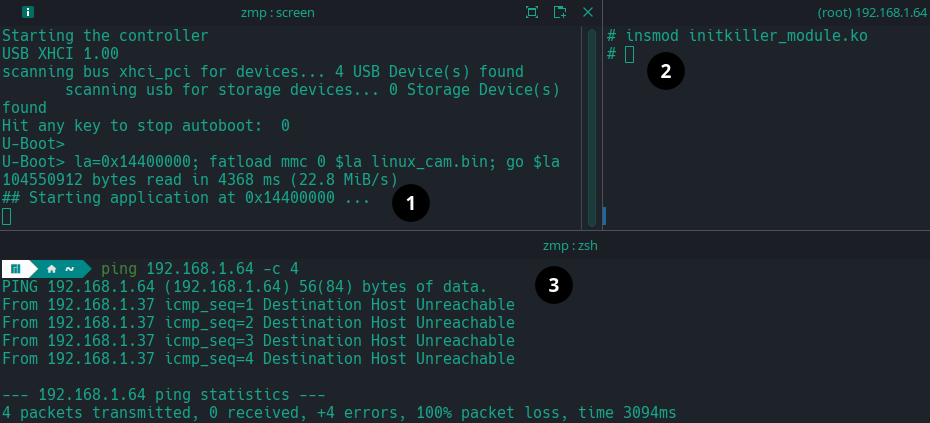
\includegraphics[width=1.0\textwidth]{./img/png/kmod-initkiller-test-annot} 
  \caption{Functional tests: testing of the kill init process kernel module -- USPFS}%
  \label{fig:kmod-initkiller-test}
\end{figure}

\begin{figure}[!hbt]
  \centering
  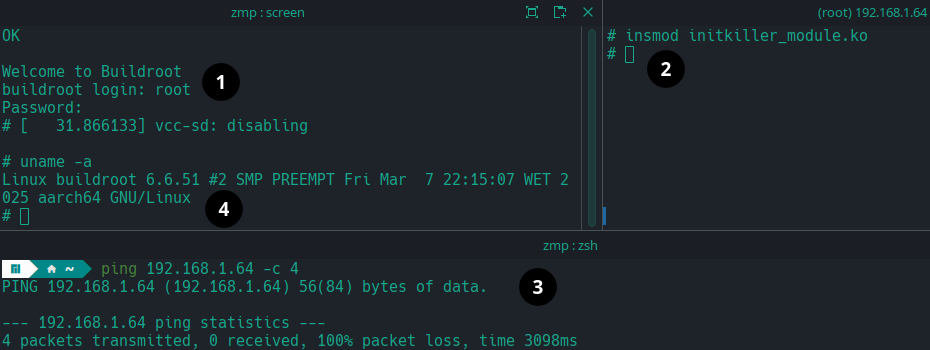
\includegraphics[width=1.0\textwidth]{./img/png/kmod-initkiller-test-bao-annot} 
  \caption{Functional tests: testing of the kill init process kernel module -- SSPFS}%
  \label{fig:kmod-initkiller-test-bao}
\end{figure}

\subsection{Unprivileged mode}
\label{sec:unprivileged-mode}
In user space the surface attack area diminishes, as the access to critical code
or hardware resources is fairly limited. Thus, one common approach is to induce
severe contention and stress on the system, which significantly impacts its
performance. Although this does not cause a literal crash of the system (unlike
the kernel module), it significantly impacts its performance. Thus, the net
effect is similar, i.e., the critical system becomes unresponsive, which can
lead to a catastrophic failure. 

Listing~\ref{lst:user-memhog} presents the implementation of a resource exhaustion
and stress application. It combines three types of attack that run in parallel: memory (lines
6--22), process (lines 25--41), and \gls{cpu} and \gls{io} (lines 43--59).
In the memory attack we perform a infinite memory allocation, while trying to
prevent the \gls{oom} killer action. In the process attack we create what is
called a ``fork bomb``, continuosly creating processes that modify a shared
memory region, after which the child process hangs (line 38). This can rapidly
overwhelm the system's process table and memory management. In the \gls{cpu} and
\gls{io} attack, we assign the highest scheduling priority to the process (line
45) to starve lower priority tasks, and then in an infinite loop (lines 52--57) we read a
page of random data to create continuous \gls{io} activity (line 63), and force
\gls{cpu} rescheduling (line 56) to increase scheduling overhead and cause extra
context switching.

To monitor the state of execution and log some relevant metrics, we added a
monitoring thread (lines 97--131), which prints: (1) the elapsed time from the
program's execution start; (2) the free
memory available (using \lstinline{sysinfo()}); (3) the number of processes
executing (from \lstinline{sysinfo.procs}); (4) the \gls{cpu} usage (calculated
using \lstinline{/proc/stat} differences); (5)
the load average (from \lstinline{sysinfo.loads}). 

In \lstinline{main()} (lines 133--157), we setup the attacks: (1) record the
start time (lines 135--136), (2) remove resource limits (lines 139--144), and
start the monitoring thread (lines 145--146). Then, the program
forks three child processes (lines 149--151): each one runs one of the three attack functions to
ensure that different system resources (memory, process table, \gls{cpu},
\gls{io}) are simultaneously stressed. Lastly, to prevent the parent process
from being terminated, an infinite loop is introduced, ensuring that it cannot be optimized by the compiler (lines 154--156).

\begin{longlisting}
\centering
% \inputminted[firstline=1, lastline=59]{c}{./listing/user_memhog.c}
\inputminted[]{c}{./listing/user_memhog.c}
\caption{Functional tests: implementation of the resource exhaustion
  application}
\label{lst:user-memhog}
\end{longlisting}

% \begin{longlisting}
% \centering
% \inputminted[firstline=61, lastline=131]{c}{./listing/user_memhog.c}
% \caption{Functional tests: implementation of the resource exhaustion
%   application -- metrics}
% \label{lst:user-memhog-2}
% \end{longlisting}

% \begin{longlisting}
% \centering
% \inputminted[firstline=61, lastline=157]{c}{./listing/user_memhog.c}
% \caption{Functional tests: implementation of the resource exhaustion
%   application -- main}
% \label{lst:user-memhog-3}
% \end{longlisting}

Fig.~\ref{fig:user-memhog-test} shows the testing of the resource exhaustion
application for the \gls{uspfs} system. In the top
left window is the \gls{uart} connection used to boot the system (1). Then, in
the top right window, we
connect remotely to \gls{uspfs} system using \gls{ssh} over Wi-Fi and start the
application in the background which periodically prints the system status (2);
we can observe the system is heavily constrained, and becomes unresponsive: even
a simple application such as \lstinline{ls} (3) cannot be executed. However,
the system does not actually crash (5), as demonstrated by the \lstinline{ping}
command. Nonetheless, the system becomes unresponsive, which would translate to a catastrophic failure of the \gls{uav}.

\begin{figure}[!hbt]
  \centering
  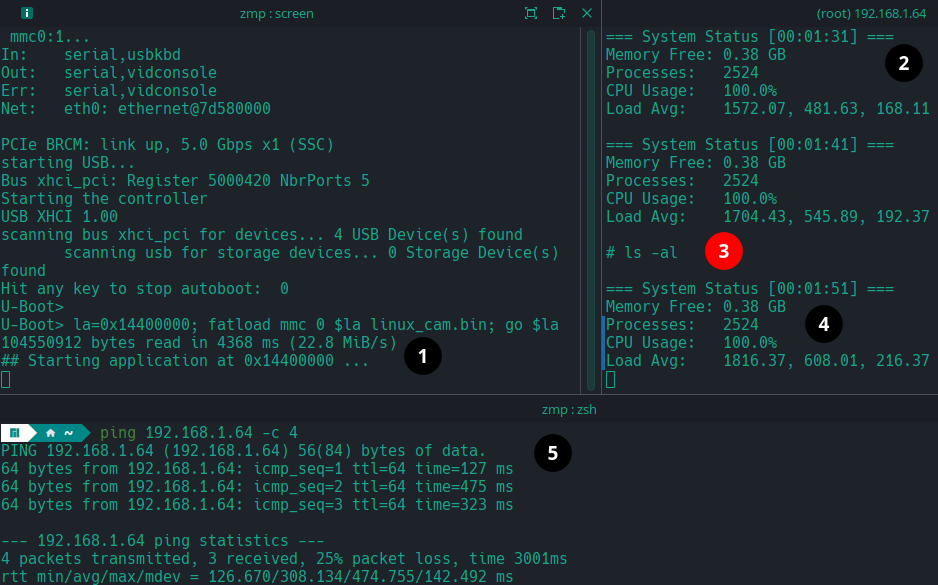
\includegraphics[width=1.0\textwidth]{./img/png/user-memhog-test-annot} 
  \caption{Functional tests: testing of the resource exhaustion application -- USPFS}%
  \label{fig:user-memhog-test}
\end{figure}


Fig.~\ref{fig:user-memhog-test} shows the testing of the resource exhaustion
application for the \gls{sspfs} system. 
In the top
left window is the \gls{uart} connection used to boot the system (1), which is
shared also between Bao and the PX4 \gls{vm}. Then, in
the top right window, we connect remotely to Companion \gls{vm} using \gls{ssh} over Wi-Fi and start the
application in the background which periodically prints the system status (2);
we can observe the system is heavily constrained, and becomes unresponsive: even
a simple application such as \lstinline{ls} (3) cannot be executed. However,
the system does not actually crash (4), as demonstrated by the \lstinline{ping}
command. 

However, we can still interact with the PX4 \gls{vm} (5), as the
Companion \gls{vm} crash does not propagate to the PX4 \gls{vm}, hence, the
\gls{uav} remains on and operational. Thus, once again, it was
demonstrated that the Bao hypervisor allows for consolidation of the
mixed-criticality software stacks
into a single platform while providing isolation between these
domains.

\begin{figure}[!hbt]
  \centering
  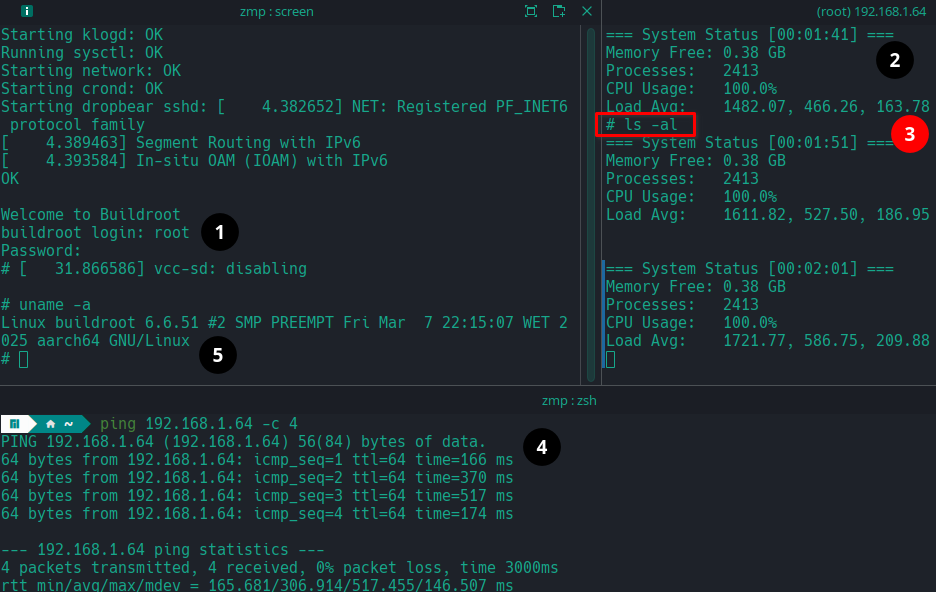
\includegraphics[width=1.0\textwidth]{./img/png/user-memhog-test-bao-annot} 
  \caption{Functional tests: testing of the resource exhaustion application -- SSPFS}%
  \label{fig:user-memhog-test-bao}
\end{figure}







\section{Bao benchmarks}
\label{sec:bao-benchmarks}
The Bao hypervisor was previously extensively benchmarked in several metrics, alongside with other
relevant hypervisors, in the context of the \gls{mcs}
applications~\cite{martins2023shedding}. Here, the same procedure is adopted,
but the focus is only in the performance assessment.

The idea is to establish the base performance of the \gls{uspfs} system (native
performance) and assess the performance degradation of the \gls{sspfs} system as
a consequence of the introduction of the Bao's hypervisor. Performance
degradation is more precisely defined as the ratio between the total execution
time of the benchmark running atop of the Bao hypervisor and native execution.

The MiBench Embedded Benchmarks' Automotive and Industrial Control Suite (AICS)
is used to benchmark the performance of the system, mimicking the environment of
embedded applications and comprises a small-scale and a large-scale variants. The former utilizes a minimized
input dataset to replicate resource-constrained execution contexts. In contrast, the latter employs an
expanded, comprehensive dataset to approximate real-world operational
conditions, facilitating rigorous assessment of performance under practical
application workloads.

The measurements tools 

Interference Workload. When evaluating memory hierarchy
interference, we use a custom baremetal guest which continuously writes a buffer with the size of the LLC (1MiB). Unless
noted otherwise, this interference guest runs on a VM with
two vCPUs. We stress that although parameterized to cause a
significant level of interference, the observed effects caused by
the interference workload do not necessarily reflect the worst
case that could be achieved if further fine-tuned.
Measurement tools. We use the Arm PMU to collect microar-
chitectural events on benchmark execution. The selected events
include instruction count, TLB accesses and refills, cache
access and refills, number of exceptions taken, and number of
interrupts triggered; we register the exception level on which
these events occur. For the Linux VMs, we use the perf tool
[45] to measure the time and to collect microarchitectural
events. For baremetal or RTOS VMs, we use the Arm Generic
Timer, with a resolution of 10 ns, and a custom PMU driver.



Fig.~\ref{fig:uav-main-eval-mibench-1} illustrates the Bao's performance
benchmarking workflow using the 
\begin{figure}[!hbt]
  \centering
  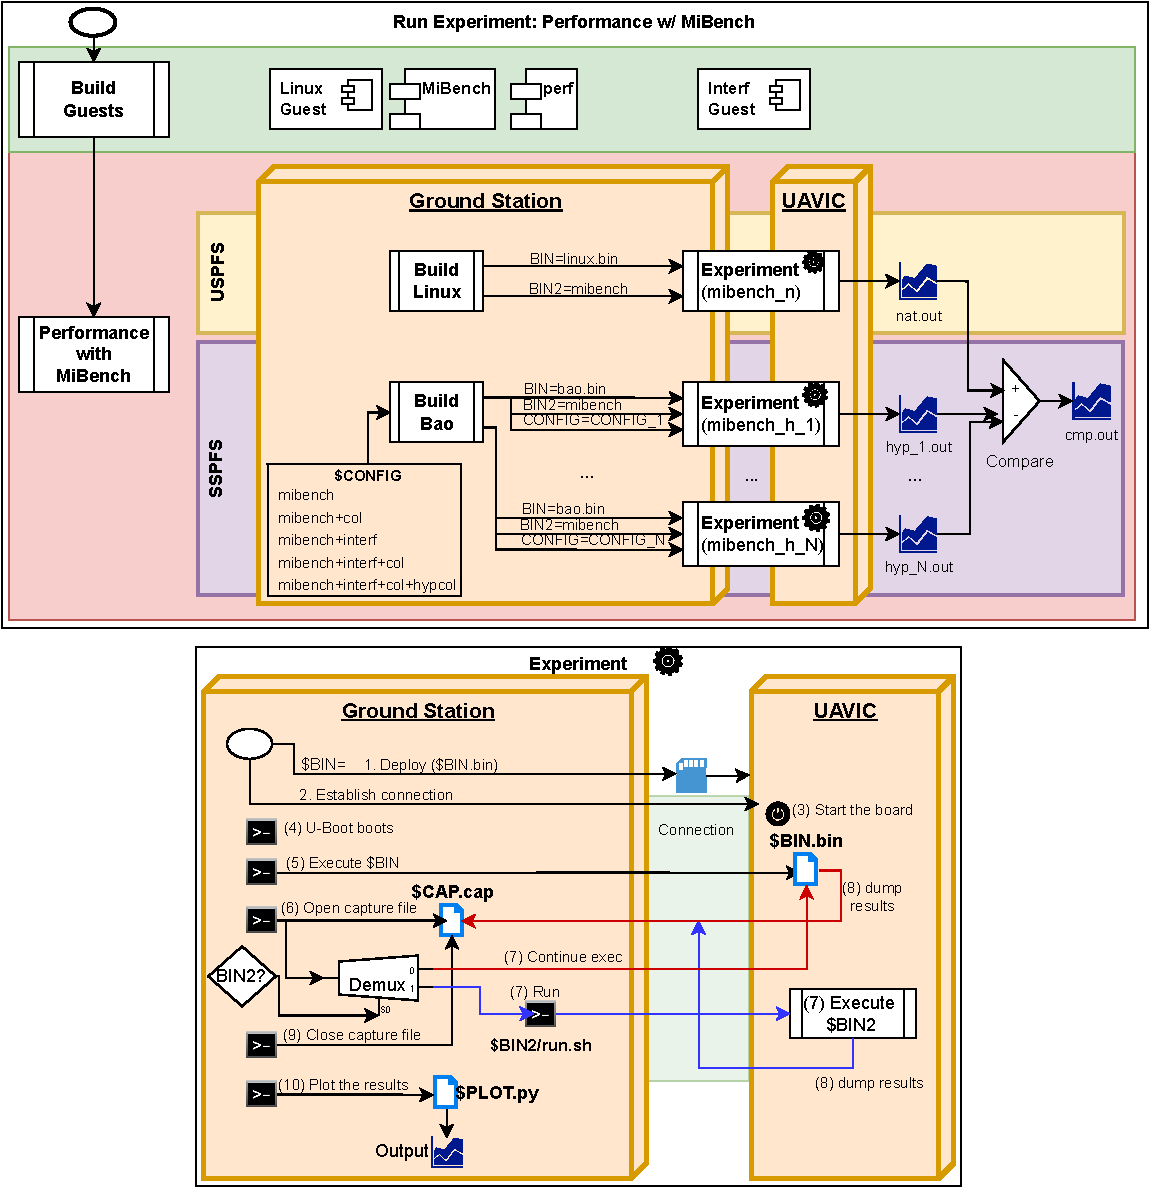
\includegraphics[width=1.0\textwidth]{./img/pdf/uav-main-eval-mibench-1} 
%  \includesvg[width=1.0\textwidth]{./img/virtualization.svg} 
  %\caption[Virtualization mind map]{Virtualization mind map}%
  \caption{Bao's performance benchmarking workflow}%
  \label{fig:uav-main-eval-mibench-1}
\end{figure}


\section{UAV benchmarks}
\label{sec:uav-benchmarks}



%%% Local Variables:
%%% mode: latex
%%% TeX-master: "../template"
%%% reftex-default-bibliography: ("../Bibliography/mieeic.bib")
%%% ispell-local-dictionary: "american"
%%% End:
